\chapter{Real Components}

Components in an Electronics 101 textbook behave very simply and predictably. In the real world, they do so only under a certain set of operating conditions. Fundamental physical properties in their construction make them behave differently in real systems. These non-ideal behaviors are called parasitic effects. This chapter will briefly describe the parasitic effects of passive components.

\section{Wires}

On a schematic a wire is a perfect conductor. Electricity flows without loss and signals experience no degredation. (To be fair, scientists are working on superconductor technologies that mimic this behavior. Currently, such systems are limited to conditions that include cooling the materials to incredibly cold temperatures.)

The most basic parasitic effect of wires is resistance. Copper, the most common wiring material, has a resistivity of $\rho = 1.68 \dot 10^{-8} \Omega m$. The next most common wiring element, aluminum, is over 50\% more resistive, but is lighter and cheaper. Silver is actually the most conductive element, beating copper by about 5\%, but is expensive and tarnishes easily. Gold is on par with aluminum for resistance, but has excellent anti-corrosion properties and thus is heavily used in connectors that get exposed to air.

When the term ``wire'' is used here, you may often think of a simple cylinder of copper in a plastic sheath that is found in the walls. In truth, all these principles apply to any conductor that is used to carry current from one point to another, including PCB traces, component leads, circuit chip bond wires, and more.

\subsection{Skin Effect}

The resistance values mentioned above are with regards to DC current. AC current is another matter: as the frequency of the current through a conductor increases, the current tends to cluster at its outside edges. This reduces the effective amount of metal that the current is flowing through, and increases the effective resistance. Figure \ref{skin_depth}\footnote{Image is in public domain. Created by Wikipedia user ``Biezl'' on 2008-July-27.} shows how high-frequency current mostly flows through the outer portion of a conductor (darker red shading is more current density).

\begin{figure}[h]
\centering
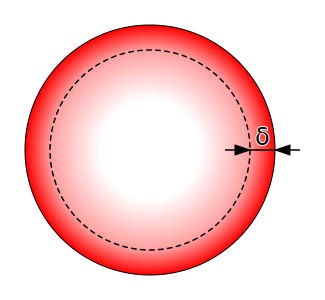
\includegraphics[scale=0.35]{skin_depth.png}
\caption{Skin Depth for HF Current}\label{skin_depth}
\end{figure}

The reason for this is how electrical current creates magnetic fields, and then those magnetic fields induce circular currents which oppose the flow of current in the wire. At its most basic level, current through a wire creates a magnetic field perpendicular to and surrounding the wire. See Figure \ref{wire_mag_field} for a simplified diagram of this effect; electrical current is in red and magnetic flux is in blue. Look up the ``right-hand rule'' for an easy way to determine the direction of the magnetic field given the current (or vice versa).

\begin{figure}[h]
\centering
\includegraphics[scale=2]{wire_mag_field.png}
\caption{Wire Current and Magnetic Field}\label{wire_mag_field}
\end{figure}

This same effect happens throughout the cross-section of a wire carrying AC current. AC current through one portion of the wire creates a magnetic field. That same field induces currents that oppose the flow of the main current in the middle of the wire, but assist the flow of current in the outer edges of the wire. An illustration of this is given in Figure \ref{skin_fields}\footnote{Image is in public domain. Created by Wikipedia user ``Biezl'' on 2008-July-27.}, with current in red and magnetic fields in blue.

\begin{figure}[h]
\centering
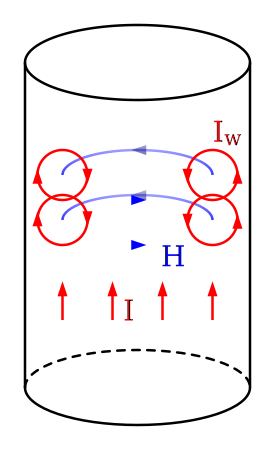
\includegraphics[scale=0.35]{skin_effect_fields.png}
\caption{Magnetic Fields In Wire}\label{skin_fields}
\end{figure}

Skin depth has a few major influencing factors. The general equation is given below (Eqn. \ref{skin_depth_eqn}). As for the terms, $\rho$ is the resistivity of the conductor, $\omega$ is the electrical frequency in radians, $\mu$ is the conductor's magnetic permeability, and $\epsilon$ is the permittivity.\footnote{Note that both the permittivity and permeability terms are products of the relative term and the free-space term. Example: $\mu = \mu_r \mu_0$.}

\begin{equation}
\delta = \sqrt{\frac{2\rho}{\omega\mu}}\sqrt{\sqrt{1+(\rho\omega\epsilon^2)}+\rho\omega\epsilon}
\label{skin_depth_eqn}
\end{equation}

As is customary, this equation is a mess. Fortunately, there's a handy simplification. At frequencies far below $\frac{1}{\rho\epsilon}$, you can ignore that double-square-root term  (leaving just the single square root term on the left). There are a few observations to make about both the full equation and its reduction.

Skin depth varies with the inverse square root of permeability. Non-ferromagnetic materials have negligible relative permeability, but ferromagnetic materials have huge permeabilities. This drastically decreases the skin depth (increasing impedance). Iron, for example, has a skin depth of less than a quarter millimeter at only 60Hz. 

Regarding the reduced equation, for good conductors like copper, the reduction is valid up into the petahertz range ($10^{15}$ Hz).

Better resistivity only helps so much at low frequencies, but at very high frequencies it can make a large difference. In the microwave region, items like waveguides can have a very thin layer of silver deposited on the outsides. The skin depth is already very small, so the 5\% boost to conductivity will help noticeably.	

Litz wire is a set of insulated conductors specially braided to counteract the skin-effect-inducing magnetic fields. It will help you avoid the problems of skin effect, but it is expensive and not often used in smaller-scale power electronics. Large grid-scale electronics may have sufficiently-high efficiency requirements to prompt the usage of Litz wire.

\subsection{Inductance}

The inductance of conductors is probably even more of a nuisance than the skin effect is, at least with modern switching power converters. There are actually several types of inductance that manifest themselves. First is the innate self-inductance of a conductor. A conductor half a millimeter in diameter (about 24AWG) has a self-inductance of about 35nH per inch.


\input{Resistors}

\section{Capacitors}

There are a few major types of capacitors you'll encounter:

\begin{itemize}
\item \emph{Aluminum Electrolytic Capacitors -} These capacitorss are one of the two workhorses of power electronics. They have huge capacitances for their size (``volumetric capacity''). They can be found in a plethora of sizes and voltage ratings. One of their drawbacks, however, is the parasitic equivalent series resistance (ESR). They almost always have noticeable ESR, and that ESR is \underline{not} stable over time and temperature. You can easily get a 15x swing over lifespan and thermal range (worst at cold temps). This causes problems in converters with electrolytic output caps because the ESR term shows up in the converter transfer function, and not in a good way. (More on this later.) Still, if you need a huge amount of capacitance, these are probably where you'll turn to. They're often paired with other types of capacitors for effective filtering.
\item \emph{Ceramic Capacitors -} These are the other type of the two workhorses of power electronics. They are in the middle ground of volumetric efficiency. They have really good (i.e. low) parasitic ESR and ESL (inductance). Tolerances and shifts over time/temp are decent. They are often use for high-frequency filtering and bypassing, and will often show up in the control circuits, too.
\item \emph{Tantalum Capacitors -} These have a lower and more predictable ESR than aluminum caps, but they are very intolerant of overvoltage conditions: they blow up. Really. They turn into mini volcanos. That's why they are practically banned in automotive applications. You'll see them in industrial and consumer stuff, however.
\item \emph{Film Capacitors -} % FINISH THIS SECTION
\item \emph{Tantalum Polymer Capacitors -} Not tantalum. Tantalum \underline{polymer}. Different. These guys have amazing volumetric efficiency, super-stable and low ESR, and nearly non-existent capacitance derating. The downside? Cost. These bastards are \emph{expensive}. Many companies choose to drop a bunch of ceramics down instead, though some are running into space constraints and have to spring for the tantalum polymer caps. You can also find aluminum polymer caps, which are halfway between aluminum electrolytic and tantalum polymer (in most every aspect).
\item \emph{Electrolytic Double-Layer Capacitors} More often called EDLC's, or SuperCapacitors, these things are unusual. The breakdown voltages are very small, with most topping out at 2.7V or so. However, the volumetric efficiency is astoundingly high. ESR decreases with case size, from worse-than-electrolytic at small SMT sizes to better-than-ceramic when you get to units as large as a beer can. Be careful with these, as the larger ones have scarily-large current capabilities.
\end{itemize}



In addition to voltage ratings, you'll often see temperature ratings such as ``X5R'' or ``Y7S'' and whatnot on ceramic capacitors. The full list for class 2 ceramic caps is given in Table \ref{class2_cer_ratings}. The first letter is the lower temperature rating. The second number is the upper temperature rating. The last digit is the maximum swing in capacitance allowable due to temperature. Note the point ``swing \ldots due to temperature.'' This is in addition to innate tolerance and voltage derating.

\begin{table}[h]
\centering
\begin{tabular}{c|c|c}
Low Temp & High Temp & Temp Tolerance \\
\hline
X = $-55^{\circ}$C & 4 = $+65^{\circ}$C & P = $\pm$10\% \\
Y = $-30^{\circ}$C & 5 = $+85^{\circ}$C & R = $\pm$15\% \\
Z = $+10^{\circ}$C & 6 = $+105^{\circ}$C & S = $\pm$22\% \\
~ & 7 = $+125^{\circ}$C & T = +22\%, -33\% \\
~ & 8 = $+150^{\circ}$C & U = +22\%, -56\% \\
~ & 9 = $+200^{\circ}$C & V = +22\%, -82\% \\
\end{tabular}
\caption{Class 2 Ceramic Capacitor Ratings}\label{class2_cer_ratings}
\end{table}

There is another class (class 1) of ceramic capacitors with the label ``NP0'' or ``C0G''. These have different material construction that results in lower volumetric efficiency but excellent tolerance and stability over voltage \& temperature. Typical tolerance swings are 30ppm$/^{\circ}$C.

\input{Inductors}

\input{Filters}

\input{Transformers}

\input{Exercises}